\chapter{Introdução}\label{sec:introducao}
O isolamento social durante o período de pandemia acabou se tornado um fator primordial no aumento dos conflitos familiares, isso obrigou a mulheres, que convivem com seus agressores, a permanecerem por um período mais longo junto a eles. Embora haja visto um aumento no número de casos de violência contra a mulher, constata-se, segundo dados da Cartilha de Violência contra a mulher de maio de 2020, que o número de denúncias diminuiu. Tal fato se dá pela proximidade da vítima ao agressor, pelo sequestro de subjetividade, pela precariedade do serviço público e pelo medo de sair do isolamento, dentre outros fatores.

\section{Escopo do Projeto}
O escopo do projeto tem como base oferecer uma aplicação simples, intuitiva e de fácil acesso ao nosso público-alvo para que estes sejam capazes de enviar um pedido de ajuda, para pessoas de sua confiança, em momentos que estiverem passando por uma situação de risco, agressão ou até mesmo violência. Estes pedidos de ajuda informarão a essas pessoas de confiança, na aplicação denominadas de “contatos seguros”, a localização atual do usuário juntamente com uma mensagem predefinida por ele.

\section{Público-alvo}
SheSafe tem como público-alvo pessoas do sexo feminino que desejam ter uma forma de comunicar a pessoas de sua confiança algum potencial risco; seja ele violência, agressão, insegurança na rua, perseguição por algum individuo ou outro risco qualquer, que estiver passando em tempo real

\section{Mapa de empatia inicial}
\begin{figure}[htbp]
  \begin{center}
  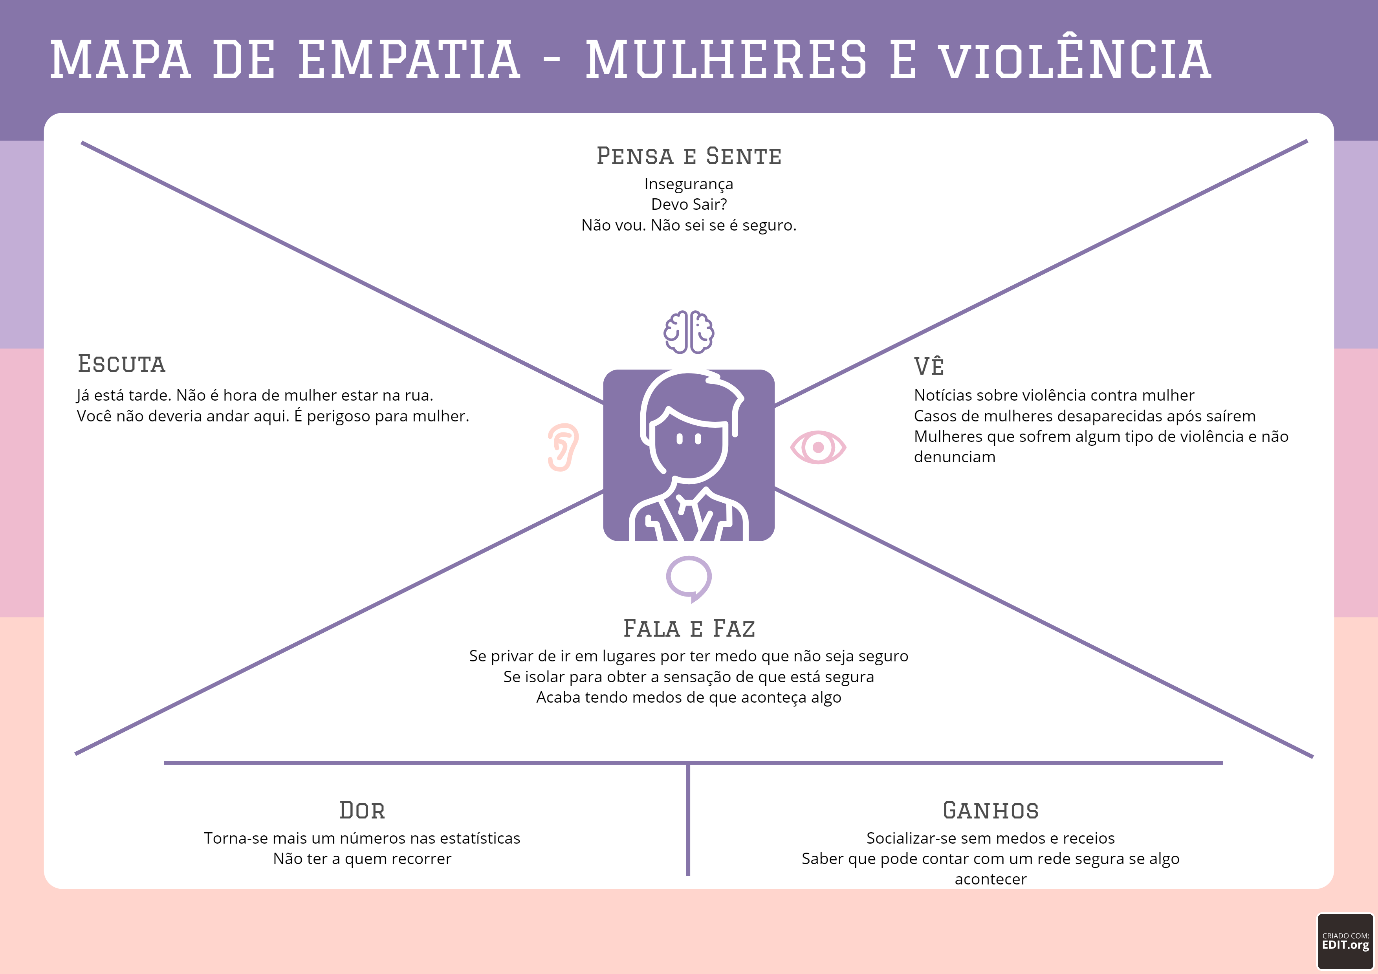
\includegraphics[width=.9\linewidth]{images/mapa-empatia-inicial.png}\\
  \end{center}
  \caption[Mapa de empatia inicial]{Mapa de empatia inicial sobre sentimento das mulheres sobre violência}
  \label{fig:mapa-empatia=inicial}
  \legend{Fonte: Próprio Autor}
\end{figure}

\section{Ambiente de uso}
O SheSafe poderá ser utilizado em qualquer ambiente desde que se tenha um plano de internet ativo para que os pedidos de ajuda possam ser enviados corretamente para a lista de contatos seguros. Uma outra restrição quanto ao uso é que os usuários devem possuir um smartphone com sistema operacional Android ou iOS para que possam instalar o aplicativo.

\section{Restrições de Uso/Circunstâncias}
Não há restrições quanto ao uso do SheSafe. Caso o usuário sinta-se em situação de risco ele poderá acionar o aplicativo e enviar seu pedido de ajuda, desde que já tenha cadastrado sua lista de contatos seguros.

\section{Diferencial}
Dado que muito dos casos de agressão acontecem com mulheres em situação de risco e muitas das vezes elas são privadas de acesso a formas de comunicação mais tecnológicas, o intuito é ter uma aplicação onde as mulheres possam reportar crimes de forma simples, prática e disponível para todos os públicos. O principal diferencial está em não restringir o acesso a aplicação para nosso público-alvo e ter a opção de envio da localização no momento do acontecimento.

\section{Funcionalidades mínimas para garantir a relevância do aplicativo}
As funcionalidades mínimas elencadas para que o projeto tenha relevância são:
\begin{alineas}
  \item Login: Para criação de usuário
  \item Pedido de socorro: Botão para acionar pedido de socorro
  \item Lista Segura: Gerenciamento de contatos seguros
  \item Perfil: Página para alteração da mensagem de socorro

\end{alineas}
